\documentclass[
	english,
	ruledheaders=section,%Ebene bis zu der die Überschriften mit Linien abgetrennt werden, vgl. DEMO-TUDaPub
	class=report,% Basisdokumentenklasse. Wählt die Korrespondierende KOMA-Script Klasse
	thesis={type=master},% Dokumententyp Thesis, für Dissertationen siehe die Demo-Datei DEMO-TUDaPhd
	accentcolor=8c,% Auswahl der Akzentfarbe
	custommargins=true,% Ränder werden mithilfe von typearea automatisch berechnet
	marginpar=false,% Kopfzeile und Fußzeile erstrecken sich nicht über die Randnotizspalte
	%BCOR=5mm,%Bindekorrektur, falls notwendig
	parskip=half-,%Absatzkennzeichnung durch Abstand vgl. KOMA-Script
	fontsize=11pt,%Basisschriftgröße laut Corporate Design ist mit 9pt häufig zu klein
%	logofile=example-image, %Falls die Logo Dateien nicht vorliegen
]{tudapub}


% Der folgende Block ist nur bei pdfTeX auf Versionen vor April 2018 notwendig
\usepackage{iftex}
\ifPDFTeX
	\usepackage[utf8]{inputenc}%kompatibilität mit TeX Versionen vor April 2018
\fi

%%%%%%%%%%%%%%%%%%%
%Sprachanpassung & Verbesserte Trennregeln
%%%%%%%%%%%%%%%%%%%
\usepackage[ngerman, main=english]{babel}
\usepackage[autostyle]{csquotes}% Anführungszeichen vereinfacht

\usepackage{microtype}
\usepackage{subfig}
\usepackage{tuda-pgfplots}
\usepackage{smartdiagram}

%%%%%%%%%%%%%%%%%%%
%Literaturverzeichnis
%%%%%%%%%%%%%%%%%%%
\usepackage[style=ieee, backend=bibtex]{biblatex}
\bibliography{Sources.bib}


%%%%%%%%%%%%%%%%%%%
%Paketvorschläge Tabellen
%%%%%%%%%%%%%%%%%%%
%\usepackage{array}     % Basispaket für Tabellenkonfiguration, wird von den folgenden automatisch geladen
\usepackage{tabularx}   % Tabellen, die sich automatisch der Breite anpassen
%\usepackage{longtable} % Mehrseitige Tabellen
%\usepackage{xltabular} % Mehrseitige Tabellen mit anpassarer Breite
\usepackage{booktabs}   % Verbesserte Möglichkeiten für Tabellenlayout über horizontale Linien


%%%%%%%%%%%%%%%%%%%
%Paketvorschläge Mathematik
%%%%%%%%%%%%%%%%%%%
%\usepackage{mathtools} % erweiterte Fassung von amsmath
%\usepackage{amssymb}   % erweiterter Zeichensatz
%\usepackage{siunitx}   % Einheiten

\let\file\texttt
\let\code\texttt
\let\tbs\textbackslash

\usepackage{pifont}% Zapf-Dingbats Symbole
\newcommand*{\FeatureTrue}{\ding{52}}
\newcommand*{\FeatureFalse}{\ding{56}}

\begin{document}

\Metadata{
	title=Pod autoscaling in Kubernetes clusters,
	author=Angelina Horn
}

\title{Pod autoscaling in Kubernetes clusters}
\author[A. Horn]{Angelina Horn}%optionales Argument ist die Signatur,
\birthplace{Bonn}%Geburtsort, bei Dissertationen zwingend notwendig
\reviewer{Prof. Dr. Felix Wolf \and Dr. Hamid Mohammadi Fard}%Gutachter

\department{inf} 
\group{Parallel Programming}

\submissiondate{\today}
\examdate{\today}

% Hinweis zur Lizenz:
% TUDa-CI verwendet momentan die Lizenz CC BY-NC-ND 2.0 DE als Voreinstellung.
% Die TU Darmstadt hat jedoch die Empfehlung von dieser auf die liberalere
% CC BY 4.0 geändert. Diese erlaubt eine Verwendung bearbeiteter Versionen und
% die kommerzielle Nutzung.
% TUDa-CI wird im nächsten größeren Release ebenfalls diese Anpassung vornehmen.
% Aus diesem Grund wird empfohlen die Lizenz manuell auszuwählen.
% \tuprints{urn=1234,printid=12345,doi=10.25534/tuprints-1234,license=cc-by-4.0}
% To see furhter information on the license option in English, remove the license= key and pay attention to the warning & help message.

% \dedication{Für alle, die \TeX{} nutzen.}

\maketitle

\affidavit[digital]
\tableofcontents

%%%%%%%%%%%%%%%%%%%
%Inhalt
%%%%%%%%%%%%%%%%%%%
\chapter{Introduction}
% Motivation
\section{Motivation}
Lately, microservice architecture is gaining popularity, especially among developers\cite{alshuqayran2016systematic}. The microservice architecture describes a new and highly flexible way of application architecture and deployment. For this approach, an application gets split into smaller but independent chunks called microservices. The created microservices will be deployed, for example as docker containers in a server cluster. These clusters will often not be maintained or owned by the applications developer but rather by an enterprise cloud provider like Google or Amazon. Microservices that belong to one deployment can communicate with one another via lightweight API interfaces e.g. REST.\\
\newline
Applications will have a dynamic load based on their workload \cite{villamizar2015evaluating}. This load however is not distributed equally among all microservices. Therefore, it is necessary to be able to scale the microservices individually while they are under load to maintain the performance of the whole application. Additionally, because of limited and costly resources, one wants to use only the minimal amount of resources that are necessary to sustain performance.\\
\newline
This can be achieved via automatic scaling \cite{rossi2019horizontal}. Automatic scaling describes a mechanism which periodically monitors every resource of a microservice, determines if and how a container should be scaled based on metrics defined by the developer and executes the scaling automatically. Because all these described architectures and ways of deployment are rather new there is room for research and improvement regarding this topic.\\
\newpage
% Objective
\section{Objective}
The objective of this thesis is to implement a novel autoscaling approach in Kubernetes to  maintain performance measured by the response time of a given microservice. Additionally, this approach should also decrease the monetary cost while possibly using public cloud resources. Therefore the objective can be divided into three separated goals:
\begin{enumerate}
	\item Depp study and research of Kubernetes and available autoscaling methods.
	\item Development and implementation of a novel autoscaling approach using machine learning.
	\item Evaluation of the developed approach, including comparison, with minimizing response time and costs in mind.
\end{enumerate}
\newpage
%%%%%%%%%%%%%%%%%%%
% Background
%%%%%%%%%%%%%%%%%%%
\chapter{Background}
In this chapter of the thesis, basic topics of which their understanding is necessary will be pointed out and explained. These topics are microservices, Kubernetes and autoscaling. Furthermore, three machine learning approaches will be explained. These topics will build the foundation and background needed for this thesis following approaches, research and statements.
% Microservices
\section{Microservices}
The term "microservice" was first introduced by James Lewis in a conference \cite{lewis2012microservices}. It describes an application architecture which is characterized by subdivided applications, that communicate with each other trough lightweight interfaces.\\ 
Each of these applications has a single responsibility or task and is deployed independently. This means that each of these microservices can be implemented in a different programming language and can be deployed on an entirely different operating system on a different server as long as they share a common interface and can communicate with each other through it. James Lewis describes this approach as "[...] rooted in the Unix Philosophy of small and simple" \cite{lewis2012microservices}.\\

\begin{figure}[h]
    \centering
    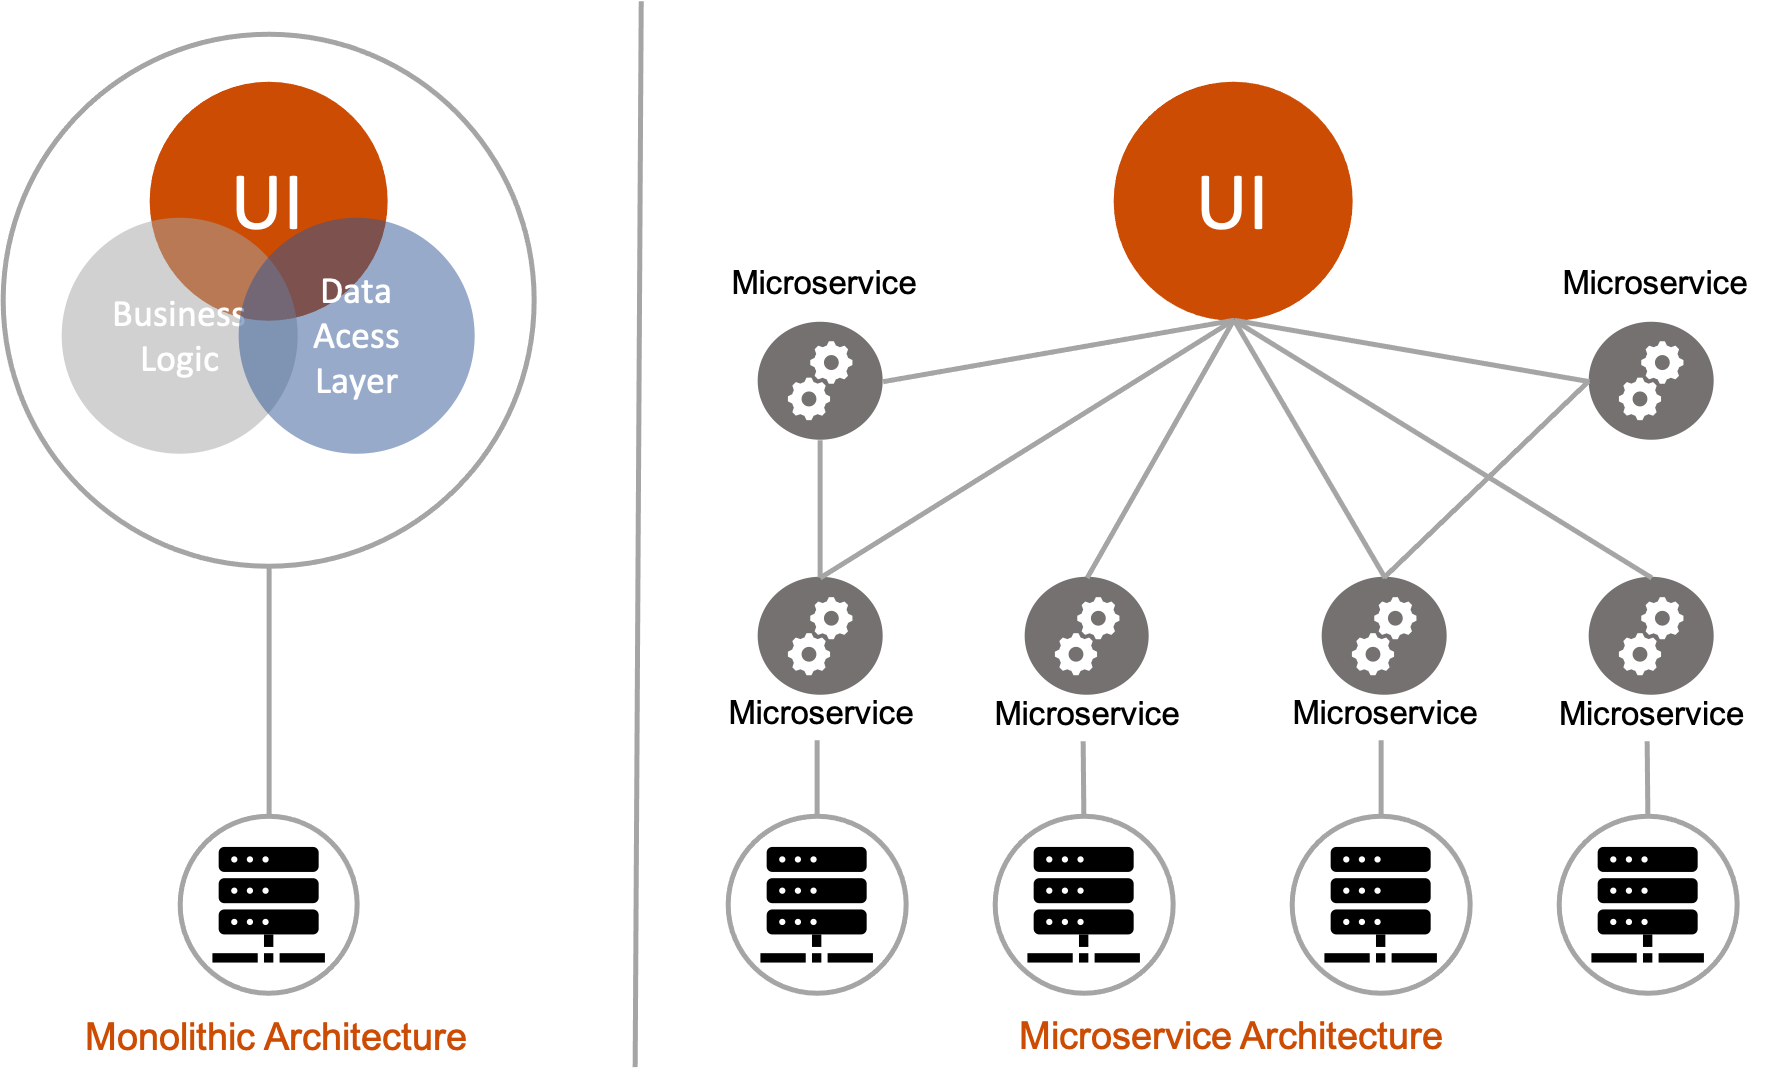
\includegraphics[width=\textwidth]{data/basics/microservice.png}
    \caption{Monolithic and microservice architectures}
    \label{fig:microservice}
\end{figure}

On one hand, this architecture offers several advantages compared to the monolithic application architecture which was popular prior (see figure \ref{fig:microservice}).
First and foremost it provides modularity which is highly beneficial regarding code complexity as well as team coordination \cite{dragoni2017microservices}. The introduction phase of new programmers is highly decreased as well as the possibilities to work on different parts of the overall application at the same time.\\

Secondly, this kind of architecture makes it possible to incrementally upgrade an application and therefore possible to reduce time to market \cite{dragoni2017microservices}. Certain parts of the application can be updated independently from the other microservices regarding not only the application code itself but also its dependencies such as libraries and environments. This way the so-called "dependency hell" \cite{merkel2014docker} which many monolithic applications suffer from can be avoided.\\

Furthermore, microservices are more resistant to failure due to their containerized existence. If one microservice fails it does not necessarily lead to the failure of the whole application. Additionally, this failed microservice can be easily restarted in a short amount of time because of its lightweight nature.\\

Last but not least, microservices introduce a new capability of scaling \cite{dragoni2017microservices, namiot2014micro}. Regarding the application, each microservice is under inconsistent load and can be scaled individually. This allows an optimal usage of resources in dependency of desired performance and costs.\\

On the other hand, this architecture brings certain disadvantages.
One major disadvantage is the time it costs to convert any application in several microservices \cite{dragoni2017microservices}. This time should not be underestimated but can also bring major benefits as stated above.
Another disadvantage is the complexity of the deployment \cite{dragoni2017microservices}. Today there are several ways to deploy microservices including the use of Jenkins\footnote{https://www.jenkins.io} or lately the use of orchestral cluster tools such as Docker Swarm\footnote{https://docs.docker.com/engine/swarm} and Kubernetes\footnote{https://kubernetes.io}.\\
% Kubernetes
\section{Kubernetes}
The term Kubernetes gained a lot of popularity over the past five years (see figure \ref{fig:google-trends-kubernetes}). It is the name of an orchestral tool for containerized applications, originally designed by Google and now owned by the Cloud Native Computer Foundation\footnote{https://www.cncf.io}. Its capabilities include deployment, scaling and monitoring of containerized microservices in clusters. These clusters can be hosted in a public or private cloud.\\
% Begin Plot
\begin{figure}[h]
    \centering
    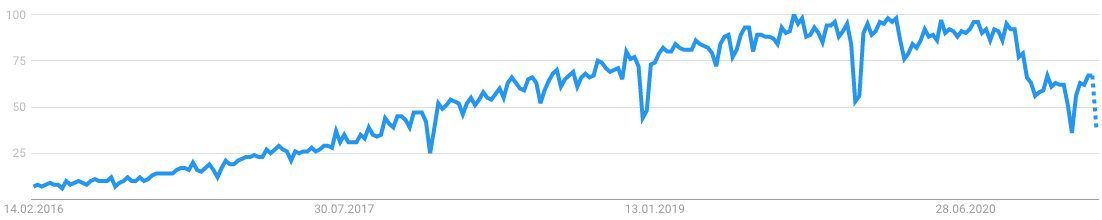
\includegraphics[width=\textwidth]{data/basics/google_trends_kubernetes.png}
    \caption{Google Trends report for the keyword "Kubernetes" \cite{googletrends2020}}
    \label{fig:google-trends-kubernetes}
\end{figure}
% Ende Plot
\begin{description}
\item[Deployment] Containerized microservices are mostly available as so-called docker images. The configuration of an application based on several microservices gets described in a "yaml" file which can be read by Kubernetes. In it several aspects of the deployment can be configured - examples are the ports on which the microservice is reachable, the number of replicas that should be deployed or the application to which the microservice belongs. Once this configuration file is made the deployment of this particular microservice is automated. 
\item[Scaling] There are two general ways to realize the scaling of a microservice. The first one is to scale a microservice manually by for example defining the resources that are available to an application or define the number of replicas in its configuration file. The second and more complex method is the automatic scaling of microservices.
\item[Monitoring] To provide stability of an application it is necessary to monitor its behavior. This enables the discovery of failures, resource use and load on the individual microservices of the application. This information is important to maintain an application. Kubernetes offers several automatic services to support maintenance. One of them is the capability to restart failed microservices according to certain settings automatically.
\end{description}

\begin{figure}[h]
    \centering
    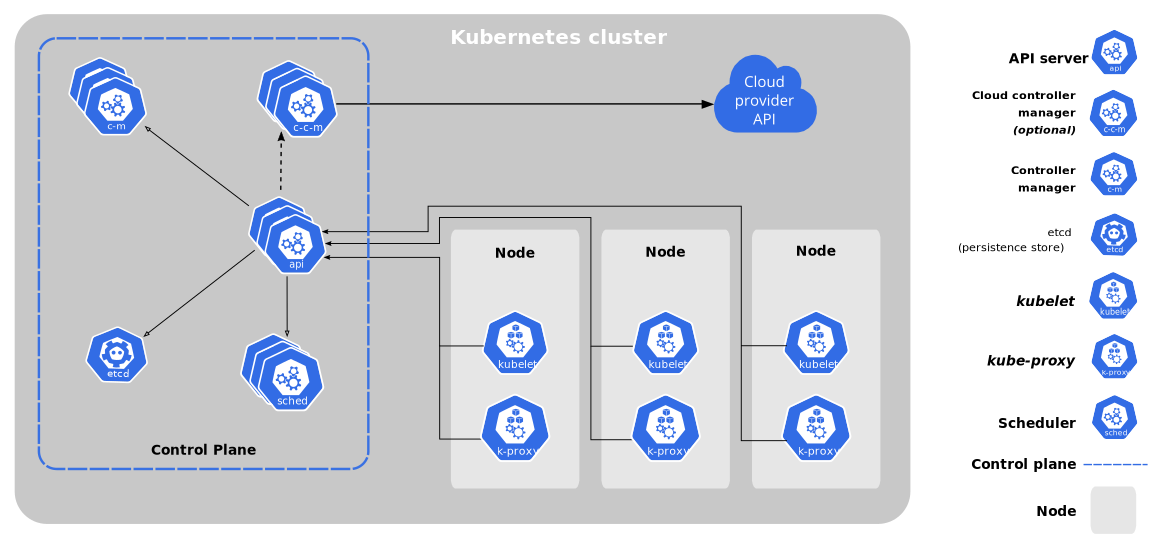
\includegraphics[width=\textwidth]{data/basics/kubernetes-cluster.png}
    \caption{Kubernetes cluster overview \cite{kubernetesdoc2020}}
    \label{fig:kubernetes-cluster}
\end{figure}

A Kubernetes cluster consists of two main structures (see figure \ref{fig:kubernetes-cluster}). The first one is called "Master" and contains the API interface, the controller manager, the scheduler and configuration storage called "etcd". The API interface is the connection point between the developer and Kubernetes. The controller manager is the executing unit of it and the scheduler plans its actions.\\ The second important structure of a Kubernetes cluster is the node. In contrary to the master there can be several nodes in a cluster. Each node contains several Pods. Each pod represents one microservice. Furthermore, each pod contains a "Kubelet" which is the executing unit of a node similar to the controller manager in the master. Additional the "cAdvisor" unit monitors the pods of a node and the "Kube-Proxy" is the connection point between a pod and the users.\\

Kubernetes offers a very powerful tool for the life cycle of an application in a cluster and paths the way for extensive development of more efficient methods to develop and maintain applications.
\newpage
% Autoscaling
\section{Autoscaling}
The term Autoscaling describes the automatic resource scaling of applications and more detailed microservices \cite{qu2018auto, midigudla2019performance}. As described in the chapter about Kubernetes: autoscaling represents the counterpart to the traditional manual scaling of applications. With this method, it is possible to allocate more resources for one microservice when it is under especially heavy load or allocate fewer resources when the load gets easier depending on its degree of use by the user.\\

\paragraph{MAPE loop}
The acronym "MAPE" stands for the terms monitor, analysis, planning and execution. They describe the basic loop that every autoscaler follows (see figure \ref{fig:mape}). The first step is monitoring. This includes fetching all the metrics that are available for a given application. The second step is to analyze the fetched data regarding for example if certain metrics exceed a given threshold. Following this, it has to be planned on how to proceed for example to increase a certain parameter. In the last step of the loop, the planned measure has to be executed. After that, the loop is completed by returning to the monitoring step. Mostly the MAPE loop is executed and repeated in a specified period.

\begin{figure}[h]
\centering
\smartdiagram[flow diagram:horizontal]{Monitor, Analysis, Planing, Execution}
\caption{MAPE loop}
\label{fig:mape}
\end{figure}

There are several methods considering and categorizing amongst other things when, how and where to scale. An organized overview gives the following taxonomy (see figure \ref{fig:autoscaling}).

\begin{figure}[h]
    \centering
    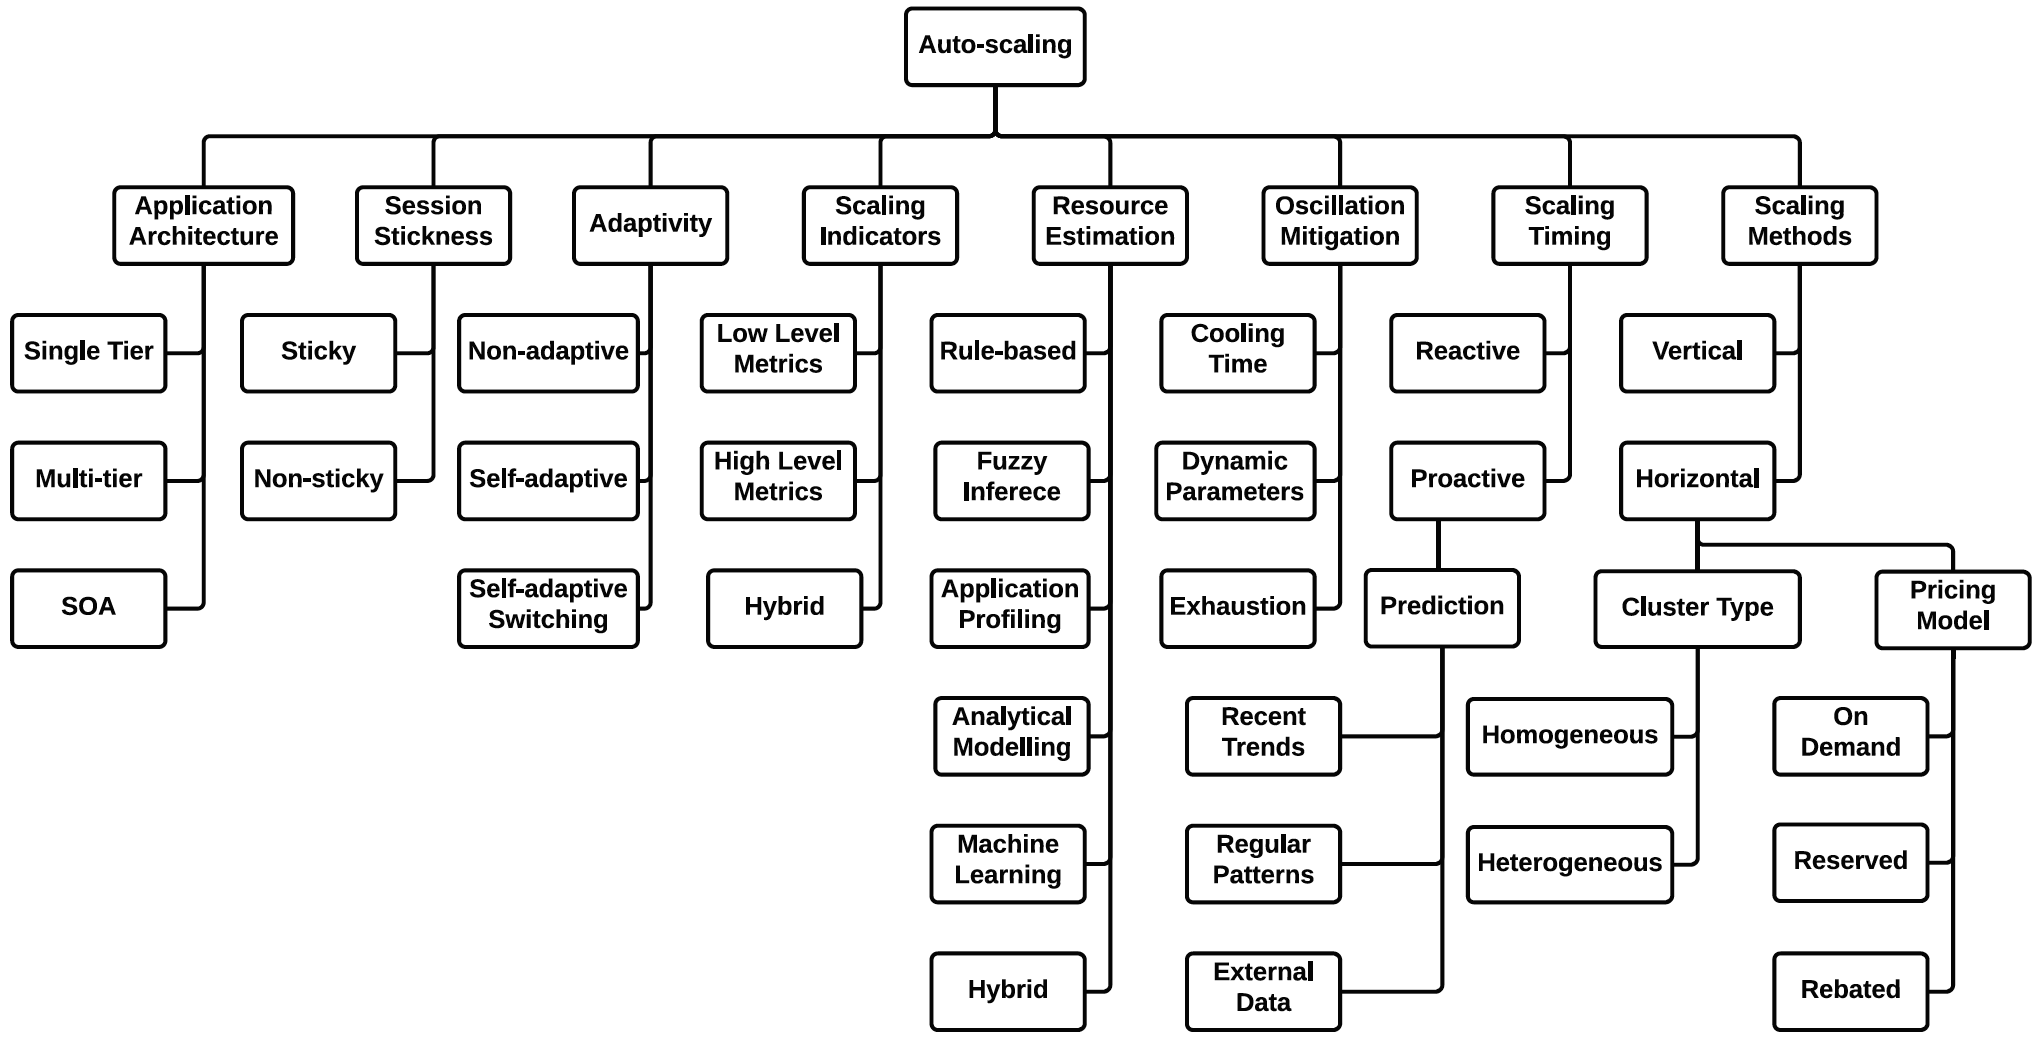
\includegraphics[width=\textwidth]{data/basics/autoscaling.png}
    \caption{Autoscaling taxonomy \cite{qu2018auto}}
    \label{fig:autoscaling}
\end{figure}

\paragraph{Scaling methods}
There are in general two types of scaling methods: horizontal and vertical \cite{qu2018auto, midigudla2019performance}.
A microservice gets scaled horizontally when its number of instances gets increased or decreased and a microservice gets scaled vertically when the resources of one instance are being increased or decreased.

\paragraph{Scaling indicators}

\paragraph{Resource estimation}
\paragraph{Scaling timing}

% Machine Learning
\section{Machine Learning}
In this chapter, a selection of related machine learning approaches are presented. Each method represents a different complexity and application level of machine learning. All of these methods will be used and compared with the same dataset later in this thesis.
% Linear Regression
\subsection{Linear Regression}
Linear Regression is originally a statistical method which attempts to model the relationship between one dependent variable and at least one independent variable \cite{montgomery2021introduction}. It does so by fitting a linear equation to the given data. The dependent variable depends on the independent or explanatory variables. The formal description of the linear equation (see \ref{eq:linear_regression}): 
\begin{equation}
Y = a + b \cdot X
\label{eq:linear_regression}	
\end{equation}
The $Y$ term represents the dependent and $X$ the explanatory variable. The value of $a$ is the y-axis intercept and $b$ is the gradient of the resulting line. There are several approaches to fitting a regression line. The basic methods are least-squares and maximum-likelihood estimation.
\paragraph{Least-Squares estimation}
The most common one is the method of least-squares. It minimizes the sum of the squares of the vertical difference from each point to the line by minimizing the quadratic loss function (see \ref{eq:quadratic_loss}). The variable $p_i$ represents the dependent variable $y_i$ corresponding point on the regression line. There are no cancellations of positive and negative values because the differences are first squared and then summed. Related methods are ordinary least-squares, weighted least-squares and generalized least-squares estimators \cite{montgomery2021introduction}.
\begin{equation}
	L = \sum_{i=1}^{N} (y_i - p_i)^2
	\label{eq:quadratic_loss}
\end{equation}

\paragraph{Maximum-likelihood estimation}
This approach searches for a set of parameters which fulfils a certain likelihood function \cite{slides_on_linear_regression}. This likelihood function represents the conditional probability to observe the given data, where a specific probability distribution and its parameters are set. This function can be interpreted as the multiplication of the conditional probability for observing each data point given the same distribution parameters. Formally this function uses the natural logarithm because of its mathematical stability and is also called the log-likelihood function (see \ref{eq:maximum_likelihood}). 
\begin{equation}
log\,L(\theta) = log\,p(X|\theta) = \sum_{n=1}^{N} log\,p(x_n|\theta)
\label{eq:maximum_likelihood}
\end{equation}

Because linear regression tries to model the relationship between certain variables, one should first determine if the relationship between these variables are of interest. This can be accomplished by for example using visualization methods like scatterplots or calculating the correlation coefficient corresponding to the given variables. A high correlation coefficient or a visible trend in the scatterplot can indicate the level of association between variables \cite{noauthor_linear_nodate, montgomery2021introduction}.\\

When the regression line is calculated, there can be data points that lie far away from the fitted line. These are called outliners. Outliners can represent for example measurement errors or indicate a not optimal regression line. These outliners can have a massive impact on the gradient of the computed line and are therefore called influential observation \cite{noauthor_linear_nodate, montgomery2021introduction}.  

\subsection{Support Vector Machines}
The Support Vector Machine theory was introduced by Vapnik of the AT\&T Bell Laboratories in 1995 \cite{vapnik1995t}. It describes a supervised machine learning model which is used for classification and regression.\\
The SVM algorithm is designed to find a hyperplane in a $n$-dimensional space which distinguishes given data points \cite{awad2015efficient}. In general, several hyperplanes are possible, but this algorithm picks the hyperplane with the constraint such that it provides the maximal distance between itself and each class of data points (see figure \ref{fig:svm}). This distance is also called margin, while the nearest data points from each class, that determine the maximal margin and therefore influence the hyperplane, are called support vectors. The dimension of the hyperplane depends on the number of features $R^{n}$. A hyperplane in for example $R^{2}$ represents a line while it represents a two-dimensional plane in $R^{3}$ \cite{awad2015efficient}.\\
% image begin
\begin{figure}[hp]%
    \centering
    \subfloat[\centering Possible Hyperplanes]{{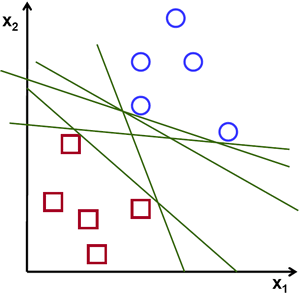
\includegraphics[width=5cm]{data/basics/svm1.png} }}%
    \qquad
    \subfloat[\centering Hyperplane with maximum margin]{{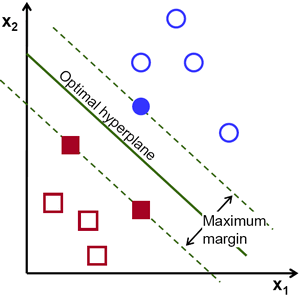
\includegraphics[width=5cm]{data/basics/svm2.png} }}%
    \caption{SVM Hyperplanes \cite{lin2017research}}%
    \label{fig:svm}%
\end{figure}
% image end
In order to handle non-linear problems it uses the kernel trick to transfer the function into higher dimensional feature space \cite{gunn1998support}. Therefore the used kernel function influences the performance of the SVM algorithm significantly and should hence be chosen wisely. The most common kernel functions are "polynomials, radial basis functions and certain
sigmoid functions" \cite{gunn1998support}.\\
\begin{figure}[hp]
\centering
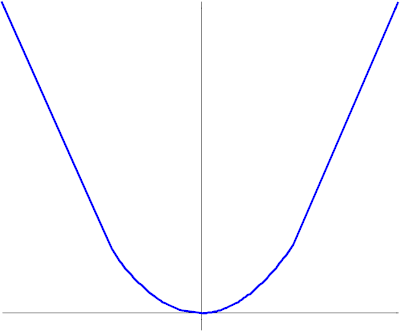
\includegraphics[width=.25\textwidth]{data/basics/svr1.png}\hfill
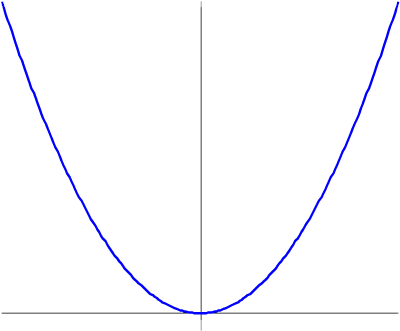
\includegraphics[width=.25\textwidth]{data/basics/svr2.png}\hfill
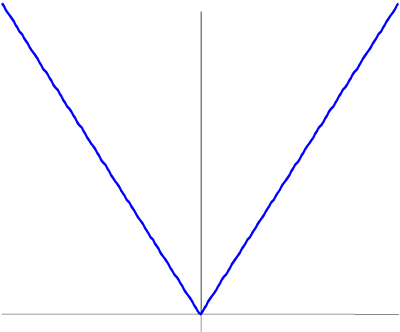
\includegraphics[width=.25\textwidth]{data/basics/svr3.png}
\caption{SVR loss functions \cite{gunn1998support}}
\label{fig:svr}
\end{figure}
Support Vector Machines can, as mentioned before, also be used for regression. To realize this, it is necessary to introduce a loss function that includes a distance measure \cite{gunn1998support}. Possible loss functions are for example Quadratic, Laplace or Huber functions (see figure \ref{fig:svr}).
\subsection{Neural Networks}
\newpage
%%%%%%%%%%%%%%%%%%%
% Related Work
%%%%%%%%%%%%%%%%%%%
\chapter{Related Work}
% absolute vs. relative metrics
\newpage
%%%%%%%%%%%%%%%%%%%
% Method
%%%%%%%%%%%%%%%%%%%
\chapter{Method}
\section{Overview}
\section{Environment Setup}
\subsection{Kubernetes}
\paragraph{Linkerd}
\paragraph{Prometheus}
\subsection{Python}
\paragraph{K8s tools}
\paragraph{Benchmark}
\paragraph{Formatting}
\subsection{Microservice}
\paragraph{Robot shop}
\section{Implementation}
\subsection{GUI}
\subsection{Benchmark}
\subsection{Machine Learning Model}
Selection of parameters
* CPU utilization
* Memory utilization
* Number of pods
Selection of metric:
* Response time
* Support Vector Machine
\subsection{Control Script}
\section{Experimentation Methodology}
comparision of performance models
\newpage
%%%%%%%%%%%%%%%%%%%
% Evaluation
%%%%%%%%%%%%%%%%%%%
\chapter{Evaluation}
\section{Results}
\section{Analysis}
\newpage
%%%%%%%%%%%%%%%%%%%
% Conclusion
%%%%%%%%%%%%%%%%%%%
\chapter{Conclusion}
\section{Summary}
\section{Outlook}
\newpage
%%%%%%%%%%%%%%%%%%%
% Bibliography
%%%%%%%%%%%%%%%%%%%
\renewcommand{\bibname}{References}
\printbibliography

\end{document}
